\documentclass[11pt,a4paper]{article}

% Pacotes essenciais
\usepackage[utf8]{inputenc}
\usepackage[T1]{fontenc}
\usepackage{lmodern}
\usepackage[portuguese]{babel}
\usepackage{graphicx}
\graphicspath{{imgs/}{imgs/base/}}
\usepackage{amsmath}
\usepackage{amsfonts}
\usepackage{amssymb}
\usepackage{float}
\usepackage{caption}
\usepackage{subcaption}
\usepackage{xcolor}
\usepackage{fancyhdr}
\usepackage{geometry}
\usepackage{titlesec}
\usepackage{lipsum}
\usepackage{cite}
\usepackage{booktabs}
\usepackage{array}
\usepackage{tikz}
\usepackage[hidelinks]{hyperref}

\newcommand{\SourceOrNote}[1]{\caption*{#1}}

% Definição das cores
\definecolor{headercolor}{HTML}{b11116}
\definecolor{secondarycolor}{HTML}{3a5461}

% Configuração da página
\geometry{
    a4paper,
    top=2.8cm,
    bottom=2.5cm,
    left=2.5cm,
    right=2.5cm,
    headheight=1.2cm,
    headsep=0.5cm
}

% Configuração do cabeçalho
\pagestyle{fancy}
\fancyhf{}
\renewcommand{\headrulewidth}{0pt}
\renewcommand{\footrulewidth}{0.5pt}

\fancyhead[L]{%
    \begin{tikzpicture}[remember picture, overlay]
        \fill[headercolor] (current page.north west) rectangle ([yshift=-1.2cm]current page.north east);
        \node[anchor=west, inner sep=0pt] at ([xshift=1cm, yshift=-0.6cm]current page.north west) 
            {
\includegraphics[height=0.8cm]{imgs/base/fatec-rgt.png}};
        \node[anchor=east, inner sep=0pt] at ([xshift=-1cm, yshift=-0.6cm]current page.north east) 
            {
\includegraphics[height=0.9cm]{imgs/base/cps-logo.png}};
        \node[anchor=east, inner sep=0pt] at ([xshift=-2.8cm, yshift=-0.6cm]current page.north east) 
            {
\includegraphics[height=1.05cm]{imgs/base/governo-sp-secretaria-logo.png}};
    \end{tikzpicture}
}

\fancyfoot[L]{\footnotesize\textcolor{secondarycolor}{Faculdade de Tecnologia do Estado de São Paulo\\ fatecregistro.cps.sp.gov.br}}
\fancyfoot[R]{\thepage}

% Configuração dos títulos das seções
\titleformat{\section}
    {\normalfont\large\bfseries\color{secondarycolor}}
    {\thesection}{1em}{}

\titleformat{\subsection}
    {\normalfont\normalsize\bfseries\color{secondarycolor}}
    {\thesubsection}{1em}{}

% Informações do artigo
\title{\vspace{0.6cm}\textbf{\Large Análise Computacional de Sistemas Complexos Utilizando Métodos Numéricos Avançados}}
\author{
    Amanda de Oliveira Costa$^{1}$, Arthur Ribeiro Dias Fudali$^{2}$, \\ Diego Baltazar de Souza Claudio$^{3}$, Giovana da Silva Albanês Santos$^{4}$, Igor Leite Gomes$^{5}$ \\[0.3cm]
    \small
    $^{1}$Faculdade de Tecnologia do Estado de São Paulo \\
    $^{2}$Universidade de São Paulo \\
    $^{3}$Instituto de Pesquisas Tecnológicas \\[0.2cm]
    \textit{amanda.costa5@aluno.cps.sp.gov.br, arthur.fudali@aluno.cps.sp.gov.br} \\
    \textit{ diego.claudio@aluno.cps.sp.gov.br, giovana.santos10@aluno.cps.sp.gov.br} \\
    \textit{igor.gomes2@aluno.cps.sp.gov.br}
}
\date{}

\begin{document}

% Força o cabeçalho em todas as páginas
\pagestyle{fancy}

\maketitle
\thispagestyle{fancy}

% Resumo
\section*{Resumo}

O Transtorno de Déficit de Atenção (TDA) é uma condição neuropsicológica que pode afetar significativamente o
desempenho de crianças em diversas esferas da vida, como estudos e relações interpessoais. O diagnóstico tradicional
envolve avaliações clínicas e testes padronizados, os quais nem sempre estão disponíveis de forma acessível ou
apresentam dados objetivos suficientes para um rastreio inicial eficaz. Este estudo propõe uma abordagem tecnológica
que integra uma plataforma digital gamificada, baseada no Teste de Desempenho Contínuo (TDC), com técnicas de
rastreamento ocular em tempo real. A proposta tem como objetivo identificar possíveis indícios de TDA em crianças
de 10 a 12 anos por meio da análise de desempenho atencional durante a execução de tarefas gamificadas. O sistema
registra dados como acertos, tempo de reação, erros de omissão e comissão, variabilidade nas respostas e padrões de
fixação ocular, os quais são processados automaticamente. Com base na comparação com bases de dados normativas,
o sistema fornece um feedback interpretativo ao usuário, podendo contribuir como ferramenta complementar de
triagem inicial. A acessibilidade da plataforma, que roda diretamente no navegador, e seu caráter lúdico e autônomo
tornam a solução promissora para ampliar o acesso ao rastreamento precoce de indícios do transtorno. A proposta
está alinhada ao terceiro Objetivo de Desenvolvimento Sustentável (ODS) da Agenda 2030 da ONU, que visa garantir
saúde e bem-estar para todas as pessoas, promovendo inovações tecnológicas para uma saúde mais inclusiva, eficiente
e orientada por dados objetivos.

\vspace{0.3cm}
\noindent\textit{\textbf{Palavras-chave:}} TDA, Atenção, Rastreamento ocular, Gamificação, ODS 3, IOT.

\vspace{0.5cm}


% Resumo
\section*{Abstract}

Attention Deficit Disorder (ADD) is a neuropsychological condition that can significantly affect children’s performance
in various areas of life, such as studies and interpersonal relationships. Traditional diagnosis involves clinical assessments
and standardized tests, which are not always readily available or provide sufficient objective data for effective initial
screening. This study proposes a technological approach that integrates a gamified digital platform, based on the
Continuous Performance Test (CPT), with real-time eye-tracking techniques. The aim is to identify possible signs of
ADD in children aged 10 to 12 years through the analysis of attentional performance during the execution of gamified
tasks. The system records data such as correct answers, reaction time, omission and commission errors, variability
in responses, and eye fixation patterns, which are processed automatically. Based on comparison with normative
databases, the system provides interpretive feedback to the user, potentially contributing as a complementary screening
tool for initial assessment. The accessibility of the platform, which runs directly in the browser, and its playful and
autonomous nature make the solution promising for expanding access to early screening for signs of the disorder. The
proposal is aligned with the third Sustainable Development Goal (SDG) of the UN’s 2030 Agenda, which aims to
ensure health and well-being for all people, promoting technological innovations for a more inclusive, efficient, and
data-driven healthcare system

\vspace{0.3cm}
\noindent\textit{\textbf{Palavras-chave:}} ADHD, Attention, Eye Tracking, Gamification, ODS 3, IOT.

\vspace{0.5cm}

\noindent\rule{\textwidth}{0.5pt}
\vspace{0.5cm}

% Introdução
\section{Introdução}

% TODO: explicar o porquê de ser destinado a profissionais testarem em crianças
A Organização das Nações Unidas (ONU) estabelece, por meio da Agenda 2030, metas para promover o desenvolvimento sustentável e o bem-estar global. Entre os 17 Objetivos de Desenvolvimento Sustentável (ODS), o terceiro busca garantir saúde de qualidade e promover o bem-estar para todos. Nesse contexto, este trabalho visa contribuir para essa meta ao propor uma solução tecnológica voltada à identificação de indícios do Transtorno de Déficit de Atenção (TDA) em crianças entre 10 e 12 anos.\cite{UN2030}

O TDA é uma condição neurobiológica de causas genéticas, que afeta milhões de pessoas em todo o mundo. É caracterizada por sintomas de
desatenção, impulsividade, e, em alguns casos, hiperatividade, afetando significativamente o
desempenho acadêmico, profissional e social dos afetados. Embora o diagnóstico clínico do
TDA seja baseado tradicionalmente em entrevistas e questionários subjetivos, avanços
tecnológicos têm permitido o uso de ferramentas mais robustas e quantitativas para apoiar
esse processo. \cite{BVS2014}
Entre essas ferramentas, destaca-se o \textit{eye tracking} (do português, rastramento ocular), esta é uma técnica
que consiste em usar o posicionamento dos olhos de uma pessoa para obter informações
sobre onde ela está olhando. Isso pode ser feito usando luzes infravermelhas, que calculam
exatamente onde a pessoa está olhando com base nas reflexões da luz na retina, ou por
meio de câmeras que monitoram visualmente a posição dos olhos e identificam sua direção.

Em ambientes controlados, o teste com eye tracking envolve a realização de tarefas
padronizadas, nas quais o comportamento visual do participante é monitorado sem
interferência direta de um moderador. Essa abordagem objetiva permite uma coleta mais
confiável de dados, reduzindo o viés associado ao autorrelato e aumentando a credibilidade
da análise. Além disso, a comparação dos dados obtidos com padrões normativos permite
identificar desvios significativos no desempenho visual atencional, muitas vezes
imperceptíveis a métodos tradicionais.

Quando aplicada em um teste diagnóstico, a técnica permite acompanhar com
precisão os movimentos dos olhos de um indivíduo durante a realização de tarefas
específicas, fornecendo dados objetivos e detalhados sobre onde, por quanto tempo e em
que sequência uma pessoa fixa seu olhar em determinados estímulos visuais. Estudos
demonstram que pessoas com TDA apresentam menor tempo de fixação e padrão visual
mais disperso ao realizarem testes de desempenho, sugerindo dificuldade em manter a
atenção sustentada e filtragem de estímulos irrelevantes \cite{Lim2024}.

A Inteligência Artificial (IA) surge como um campo essencial nesse contexto, voltado à criação de sistemas capazes de simular aspectos da cognição humana, como percepção, raciocínio, aprendizado e tomada de decisão. Segundo \cite{sep-chinese-room}, a IA pode ser dividida em dois tipos: IA Forte, capaz de compreender e raciocinar de forma semelhante aos humanos; e IA Fraca, restrita à execução de tarefas específicas sem capacidade de raciocínio autônomo. O avanço dessas tecnologias, apoiado por algoritmos de aprendizagem profunda, processamento de linguagem natural e análise de dados, tem permitido desenvolver sistemas cada vez mais precisos e adaptativos.

Associada à IA, a Internet das Coisas (Internet of Things, IoT) amplia o potencial de integração tecnológica ao conectar dispositivos físicos, como sensores e equipamentos inteligentes, à internet. Essa interconexão possibilita a coleta, o compartilhamento e a análise de dados em tempo real, criando ecossistemas inteligentes baseados em computação em nuvem e comunicação entre máquinas. \cite{IEEE}
 
O Teste de Desempenho Contínuo (TDC) é uma medida padronizada amplamente
utilizada na neuropsicologia para avaliar métricas de atenção sustentada, impulsividade,
tempo de resposta e variabilidade dos tempos de reação. Trata-se de uma tarefa
computadorizada na qual o usuário responde e reage a estímulos apresentados
sequencialmente, permitindo medidas de desempenho atencional ao longo do tempo. 
A atenção é um processo cognitivo complexo que envolve diferentes componentes inter-relacionados, essenciais para o desempenho em tarefas como o teste de desempenho contínuo. De forma geral, pode ser classificada em quatro tipos principais. A atenção sustentada refere-se à capacidade de manter o foco em um estímulo ou tarefa por um período prolongado, sendo fundamental para evitar erros de omissão no TDC. A atenção seletiva envolve a habilidade de concentrar-se em informações relevantes enquanto se ignora distrações, o que influencia diretamente a precisão das respostas. A atenção alternada diz respeito à flexibilidade cognitiva para mudar o foco entre diferentes estímulos ou tarefas, demonstrando controle executivo. Por fim, a atenção dividida representa a capacidade de processar simultaneamente múltiplas fontes de informação, exigindo coordenação eficiente de recursos cognitivos. A compreensão dessas modalidades permite interpretar de forma mais abrangente as métricas obtidas no TDC. \cite{CULLUM1998303}

Os \textit{serious games} (jogos sérios) também vêm se destacando como ferramentas complementares em contextos de avaliação e reabilitação cognitiva. Esses jogos digitais, desenvolvidos com finalidades que vão além do entretenimento, oferecem ambientes interativos e imersivos que aumentam o engajamento do usuário e permitem mensurar habilidades cognitivas de forma dinâmica.

Desta forma,a integração entre eye tracking, IA e jogos sérios representa uma abordagem promissora para a triagem e o apoio diagnóstico do TDA.
A análise dos dados com IA pode indicar o grau de
desatenção apresentado por um indivíduo em diferentes contextos e contribuir para decisões
clínicas mais embasadas. Assim, este estudo propõe o desenvolvimento de um software gamificado que utilize informações de rastreamento ocular processadas com base nas métricas do TDC, a fim de gerar um indicador do desempenho atencional geral e oferecer uma possível estimativa preliminar para o Transtorno de Déficit de Atenção.

% Objetivo
\section{Objetivo}
Desenvolver uma plataforma digital gamificada, acessível por navegador, que utiliza
rastreamento ocular e métricas de desempenho atencional para auxiliar na triagem inicial de
indícios do TDA em crianças de 10 a 12 anos.

\subsection*{OBJETIVOS ESPECÍFICOS} 

\begin{itemize}
    \item Integrar o TDC a um jogo digital com tarefas que
    simulam desafios atencionais.
    \item  Aplicar técnicas de \textit{eye tracking} em tempo real para registrar padrões de
    atenção durante a execução das tarefas.
    \item Processar automaticamente os dados coletados e compará-los com parâmetros
    normativos para gerar feedback ao usuário.
    \item Promover uma solução acessível, autônoma e alinhada ao ODS 3 da ONU, que amplie
    o acesso à triagem inicial de TDA.
\end{itemize}


% Estado da Arte
\section{Estado da Arte}

O diagnóstico do TDA em adultos continua sendo
um desafio clínico significativo. Tradicionalmente, o processo diagnóstico baseia-se em
entrevistas e testes clínicos, autorrelato e relatos de informantes, instrumentos que, embora
úteis, podem ser afetados por viés retrospectivo, subjetividade do paciente, e simulação dos
testes, resultando em casos de falsos positivos ou negativos. Dessa forma, o interesse por
abordagens objetivas e tecnologicamente assistidas, que combinem dados neuropsicológicos
e comportamentais com técnicas de análises automatizadas, aumentou. Estudos recentes
têm investigado o uso de jogos digitais sérios como ferramentas de avaliação e treinamento
cognitivo, com foco na atenção contínua. \cite{Nascimento2020} exploraram a relação
entre a prática regular de videogames e o desempenho em atenção sustentada, avaliado
pelo \textit{Conners’ Continuous Performance Test II} (CPT II), uma versão amplamente utilizada do
TDC. Embora não tenham encontrado diferenças de
performance entre jogadores de videogames de ação, não ação e não jogadores, os autores
identificaram o sexo como uma variável relevante, pois notara diferença entre tempo de
reação e número de erros. O estudo destaca a complexidade das interações entre fatores
individuais e experiências digitais, sugerindo que a aplicação de jogos, mesmo quando
classificados como serious games, precisam de cuidados na metodologia e no controle de
variáveis, com o fim de evitar interferências no desempenho atencional.

Nesse contexto, \cite{Elbaum2020} exploraram o potencial diagnóstico da integração
entre o \textit{MOXO-dCPT} (um TDC com fases estruturadas de distrações
auditivas e visuais) e dados de \textit{eye tracking}. O estudo contou com uma
amostra de 85 adultos (43 com diagnóstico formal de TDAH e 42 controles saudáveis) e
analisou o padrão de atenção visual ao longo de diferentes partes do teste. Os resultados
demonstraram que indivíduos com TDAH apresentaram maior tempo de fixação em áreas
irrelevantes da tela, particularmente em condições com distrações visuais, o que os autores
interpretaram como uma medida direta de distratibilidade atencional objetiva. Essa métrica
comportamental demonstrou maior poder discriminativo em comparação às melhores
pontuações tradicionais do \textit{MOXO}. Além disso, os autores propuseram que as partes do teste
com distrações visuais poderiam ser utilizadas isoladamente, reduzindo o tempo do teste e
mantendo a precisão.

Avançando nesse campo, \cite{Wiebe2024} criaram uma solução diagnóstica que
envolve um ambiente de realidade virtual (VR), onde os participantes realizavam um teste de
desempenho imersivo sob a ocorrência de distrações simuladas em um ambiente 3D.
Durante a tarefa, foram coletados dados simultâneos de eye tracking, movimentos da
cabeça, eletroencefalograma (EEG) e desempenho atencional. O modelo de IA (inteligência Artificial) foi treinado
em um conjunto de 50 participantes e testado de forma independente em outro conjunto de
36 indivíduos. O modelo final, com apenas 11 variáveis selecionadas, alcançou 81\% de
acurácia, 78\% de sensibilidade e 83\% de especificidade no conjunto de teste.

Os estudos indicam que a utilização de tecnologias de rastreamento ocular, tarefas
cognitivas com análises embasadas dos dados representam um avanço significativo em
relação aos métodos tradicionais de diagnóstico. O uso de \textit{serious games} para coleta de
dados de desempenho também é eficaz, como mostra o trabalho de Nascimento e Menezes.
O trabalho de \cite{Elbaum2020}. oferece um modelo aplicável e eficiente ao integrar eye tracking
em um teste comercial já existente, o estudo de \cite{Wiebe2024}. diferencia a proposta ao
incorporar realidade virtual, aprendizado de máquina e validação externa em amostras
independentes. Juntos, os estudos reforçam a ideia de que sistemas digitais automatizados
podem melhorar a precisão diagnóstica do TDAH em adultos.


% Metodologia
\section{Metodologia}



A \textit{landing page} do projeto foi desenvolvida em \textit{HTML}, responsável pela estrutura do conteúdo, \textit{CSS}, utilizado para o estilo visual, e \textit{JavaScript}, empregado na implementação da interatividade e do dinamismo da navegação. O sistema de rastreamento ocular foi implementado em JavaScript, utilizando a biblioteca \textit{WebGazer.js}, que contém um modelo capaz de se autocalibrar ao observar a interação dos visitantes com a página, treinando um mapeamento entre as características do olhar e as posições na tela \cite{papoutsaki2016webgazer}. O tratamento das coordenadas oculares recebidas do \textit{frontend} foi realizado em \textit{JavaScript}, com o uso do \textit{Node.js} e do \textit{Socket.IO}, possibilitando a comunicação em tempo real com o frontend, uma vez que depende das coordenadas enviadas por ele. Essa parte do \textit{backend} é responsável por analisar as métricas TDC (acertos e erros), dados que serão utilizados para compor o feedback individual de cada usuário. No backend, a biblioteca serialport gerencia a comunicação serial pela porta COM \textit{(Windows)}, enviando comandos ao dispositivo \textit{IoT} e recebendo eventos, integrados ao frontend em tempo real via Socket.IO. Por fim, o jogo \textit{web} foi desenvolvido em \textit{TypeScript}, utilizando o \textit{framework} \textit{Next.js}, o que proporcionou um código mais robusto, organizado e uma experiência de uso moderna e fluida.

Optou-se pela utilização do banco de dados não relacional \textit{MongoDB}, o qual armazena informações em documentos no formato \textit{JSON}, possibilitando a criação de estruturas dinâmicas e aninhadas, adequadas ao armazenamento dos dados provenientes dos testes de rastreamento ocular. Sua flexibilidade e escalabilidade o tornam mais apropriado que bancos relacionais para o tratamento de grandes volumes de dados sensoriais. O gerenciamento do banco foi realizado por meio do \textit{MongoDB Compass}, ferramenta que facilita a execução de consultas, validação de esquemas e análise de desempenho.

TODO: ADD PARTE DE CLOUD

A metodologia fundamenta-se na aplicação adaptada do Teste de Desempenho Contínuo, tarefa computadorizada amplamente utilizada em psicologia e neuropsicologia para avaliar atenção e controle inibitório. Ao contrário de questionários, exige respostas comportamentais em tempo real e produz métricas objetivas como acertos, erros de omissão e comissão, tempo de reação e variabilidade das respostas. Optou‑se por seguir a lógica de estudos como //TODO: COLOCAR REF, nos quais os participantes observam um fluxo contínuo de estímulos e respondem a um sinal‑chave; essa dinâmica foi adaptada às três fases do jogo, cada uma com características próprias.

A principal contribuição deste estudo consiste na integração do TDC ao rastreamento ocular em tempo real para avaliar o nível de atenção, o que contribui como auxílio ao pré-diagnóstico do TDA. Ao registrar variáveis de olhar, por exemplo, duração de fixação, dispersão do olhar e tempo sobre alvos, busca‑se complementar as medidas comportamentais do teste e aumentar a confiabilidade da avaliação. Essas medidas oculares apresentam menor dependência da resposta deliberada do participante, pois capturam sinais contínuos e fisiológicos da atenção que podem ser sincronizados com os eventos do exame. Dessa forma, é possível detectar padrões que contribuem com a interpretação clínica. Ressalta‑se, contudo, que o rastreamento ocular é complementar e não substitui a avaliação clínica.

O estudo é estruturado como um jogo digital de temática espacial, composto por três fases com níveis crescentes de dificuldade. A mecânica do jogo foi elaborada para simular os princípios do TDC, promovendo a exposição contínua a estímulos visuais por períodos prolongados e exigindo respostas rápidas e consistentes por parte do participante. O jogo será aplicado por profissionais da saúde, como psicólogos, para a triagem inicial de indícios de TDA em crianças entre 10 e 12 anos. O ambiente de teste é controlado, com supervisão profissional, o que garante a padronização das condições de aplicação e a segurança dos participantes.

Com o objetivo de aprofundar a compreensão do tema e promover um alinhamento mais preciso entre os aspectos técnicos e psicológicos do projeto, foi conduzida uma pesquisa de campo com quatro profissionais da área da Psicologia. As entrevistas buscaram avaliar a viabilidade técnica da proposta, identificar os sintomas mais recorrentes do TDA e compreender os tipos de estímulos que mais influenciam os processos de distração em indivíduos com esse transtorno.

A análise qualitativa dos dados revelou que estímulos visuais e auditivos, especialmente movimento, cor e som, exercem papel determinante na indução de distrações, devendo, portanto, ser considerados elementos centrais no planejamento das fases experimentais. Adicionalmente, pode-se citar a instrução de avisar os jogadores sobre as distrações. Nas fases um e três, durante as instruções, os participantes são avisados sobre os distratores e orientados a não olhar para eles, pois esta ação impacta negativamente a pontuação, já que o objetivo dessas fases é que a criança mantenha o foco nos alvos, ignorando os distratores. 

Além disso, os profissionais destacaram a importância de incluir uma etapa em que os distratores estejam presentes de forma indireta, sem que o participante seja instruído a focar neles, semelhante ao teste citado em // TODO: COLOCAR REF DO VÍDEO. Nesse teste, a instrução inicial é contar quantos passes de bola o time de branco realiza, ao final, após a resposta, uma pergunta adicional questiona se o participante observou uma distração (urso dançando) durante o jogo de basquete. Dessa forma, o participante não procura pela distração, mas, caso consiga detectá-la, infere-se que impacta positivamente no pré-diagnóstico, pois a instrução inicial direcionava o foco para os alvos, tornando a distração menos atraente. De forma análoga, na fase 2 do jogo, os planetas transitam pela tela sem que o participante seja instruído a observá-los. 

Para uma melhor compreensão do funcionamento do sistema, a Figura \ref{fig:fluxograma} apresenta o fluxograma do processo, que descreve a sequência lógica das operações realizadas pelo sistema até o término das três partidas. 

\begin{figure}[H]
    \centering
    \caption{Fluxograma do sistema}%
    \label{fig:fluxograma}
    
\includegraphics[width=\textwidth]{fluxograma.png}%
    \SourceOrNote{Autoria Própria (2025)}
\end{figure}

Na etapa 1, ocorre a calibração dos olhos do jogador, processo em que o sistema identifica e ajusta os pontos de fixação ocular do usuário antes do início do jogo, garantindo a precisão do rastreamento. Em seguida, é executada a coleta das métricas TDC, que ocorre automaticamente durante as três fases do jogo. Nessa etapa, o sistema processa e registra parâmetros como número de acertos, erros de omissão, erros de comissão, tempo de reação e variabilidade temporal das respostas. Na etapa 2, há uma tomada de decisão para verificar se o participante irá jogar no modo de treinamento. Caso o modo de treinamento esteja habilitado (etapa 3), o sistema armazena as métricas TDC em uma base de dados, permitindo que o módulo de treinamento da IA realize a análise comparativa entre os dados do indivíduo e a base existente. Esse processo visa aprimorar o modelo e gerar um pré-diagnóstico personalizado. Já na etapa 4, quando o modo de treinamento não está ativado, o sistema realiza diretamente a geração e exibição do pré-diagnóstico, utilizando as métricas coletadas durante a execução do jogo. 

Durante toda a experiência, o rastreamento ocular é realizado em segundo plano, utilizando a biblioteca WebGazer.js para capturar os pontos de fixação visual do usuário por meio da \textit{webcam Logitech Brio Cam HS}. Para garantir a precisão da predição do olhar, a WebGazer.js utiliza uma arquitetura que combina diferentes técnicas de Aprendizado de Máquina. Inicialmente, o \textit{TensorFlow FaceMesh} é mobilizado para a detecção precisa e em tempo real da face e, especificamente, dos pontos de referência da região ocular. O modelo de predição propriamente dito é baseado na Regressão Ridge, que é uma variação da regressão linear. A principal função desta técnica é atuar como um mecanismo de regularização, que, simplificadamente, evita o superajustamento \textit{(overfitting)} do modelo. Isso significa que ela impede que o modelo fique muito focado nos dados de treinamento, o que faria com que ele errasse ao lidar com novos usuários. A Regressão Ridge faz isso aliviando a influência dos parâmetros de maior valor no aprendizado. O resultado é um modelo mais robusto e generalizável, capaz de realizar o mapeamento entre a imagem dos olhos e as coordenadas da tela de forma confiável para diferentes participantes. Finalmente, no pós-processamento, as predições de olhar bruto são submetidas ao Filtro de Kalman, um algoritmo recursivo que suaviza os dados, aumentando a fluidez e a estabilidade da predição ao estimar o próximo ponto de fixação com base na observação anterior \cite{WebGazerDoc}.É importante notar que todos os componentes algorítmicos, incluindo \textit{FaceMesh}, Regressão Ridge e Filtro de Kalman, são nativos da biblioteca WebGazer.js e foram empregados em sua configuração padrão, sem modificações.

Os dados de fixação visual coletados permitem identificar padrões de atenção ou desatenção, que são contrastados com nossa base de dados em cada etapa da atividade. Em paralelo à coleta desses dados, todas as fases do experimento são configuradas para potencializar a sobrecarga sensorial e dificultar a concentração do participante. Para tal, utilizam-se música de fundo, cuja intensidade e ritmo são ajustados conforme o nível de dificuldade, e a imposição de um tempo máximo definido, elementos que, em conjunto, intensificam o estresse cognitivo e a exigência da tarefa.

O profissional, já com cadastro e login previamente definidos na plataforma, assim como a criação do perfil do paciente que irá jogar, pode acessar o sistema. O participante é direcionado para a página de instruções, onde são apresentadas a sequência de como calibrar o olhar para poder prosseguir para o jogo.

\begin{figure}[H]
    \centering
    \caption{Calibração do olhar}%
    \label{fig:calibracao}
    
\includegraphics[width=\textwidth]{calibracao.png}%
    \SourceOrNote{Autoria Própria (2025)}
\end{figure}

A calibração é realizada antes do início do jogo, de modo que o sistema ajuste o mapeamento entre as características do olhar e as posições na tela. O procedimento inclui nove pontos de fixação (estrelas) dispostos em uma grade 3×3. O participante é instruído a fixar o olhar em cada ponto por cerca de cinco segundos e a posicionar o cursor sobre a estrela, clicando nela até que esta desapareça; simultaneamente, o sistema registra as coordenadas oculares. Esse procedimento é essencial para compensar variações individuais na anatomia, postura e distância da câmera, garantindo maior precisão do rastreamento. Concluída a calibração, o sistema encontra‑se apto a interpretar os movimentos oculares durante as fases do jogo.

Antes de cada fase, existem as instruções da mesma. Em seguida, o usuário inicia a primeira etapa do teste. 

\begin{figure}[H]
    \centering
    \caption{Primeira fase}%
    \label{fig:primeira-fase}
    
\includegraphics[width=\textwidth]{primeira-fase.png}%
    \SourceOrNote{Autoria Própria (2025)}
\end{figure}

Na primeira fase, o participante deve fixar o olhar por cinco segundos em cinco alvos estáticos, representados por estrelas, enquanto elementos animados surgem ao redor. Após os cinco segundos, cada estrela desaparece da tela. A música de fundo apresenta ritmo moderado e a duração total da fase é de um minuto. O objetivo é avaliar a capacidade de manter a atenção em um ponto fixo, ignorando estímulos visuais e auditivos periféricos.

Nesta fase, foram aplicados procedimentos de atenção sustentada, manter foco em um estímulo por um período prolongado e, atenção seletiva, manter o foco em um estímulo relevante, ignorando distrações, conforme recomendado pelos profissionais entrevistados. Além disso, a técnica proposta por // TODO: COLOCAR REF, na qual os participantes observam um fluxo contínuo de estímulos (estrelas) e respondem a um sinal‑chave (estrela acesa), ou seja, a resposta deve ser direcionada ao alvo previsto.

Ao iniciar a fase, estabelece-se uma conexão via \textit{WebSocket} entre o cliente (front-end) e o servidor (back-end). Em seguida, o servidor identifica o cliente conectado, que envia as coordenadas das estrelas para o endpoint $\texttt{/iniciar\_fase1}$. O processo de \textit{eye tracking} é então iniciado, e o cliente passa a transmitir as coordenadas dos olhos a cada 1 segundo para $\texttt{/gaze\_data\_fase1}$. Paralelamente, o servidor seleciona uma das cinco estrelas como alvo atual, enquanto o cliente permanece em escuta por meio de $\texttt{/fase1\_iniciada}$, responsável por destacar a estrela correspondente e manter o envio das coordenadas oculares. Esse procedimento se repete até que todas as estrelas sejam visualizadas por, no mínimo, 5 segundos, de modo que o participante fixe o olhar no alvo até sua desaparecimento da tela. Ao final da fase, o servidor salva o objeto $\texttt{ExperimentosFase1Schema}$ no banco de dados, contendo as informações do paciente, a data e a hora do teste, um array do histórico de olhar da criança, com o alvo, as coordenadas e o estado de fixação, além de um array com o resultado de cada alvo, indicando métricas de tempo e o motivo do término. Após o armazenamento desses dados, o servidor calcula as métricas TDC da fase 1, a saber: número de acertos (fixação por 5 segundos), número de erros de omissão (demora de 10 segundos ou mais para iniciar a fixação) e erros de comissão (início da fixação antes de 10 segundos, sem manutenção do foco por 5 segundos). Essas métricas são enviadas ao cliente por meio de $\texttt{/fase\_concluida}$, permitindo que o usuário visualize seu desempenho na fase, conforme ilustrado na Figura \ref{fig:fim-primeira-fase}.

\begin{figure}[H]
    \centering
    \caption{Resultados da fase 1}%
    \label{fig:fim-primeira-fase}
    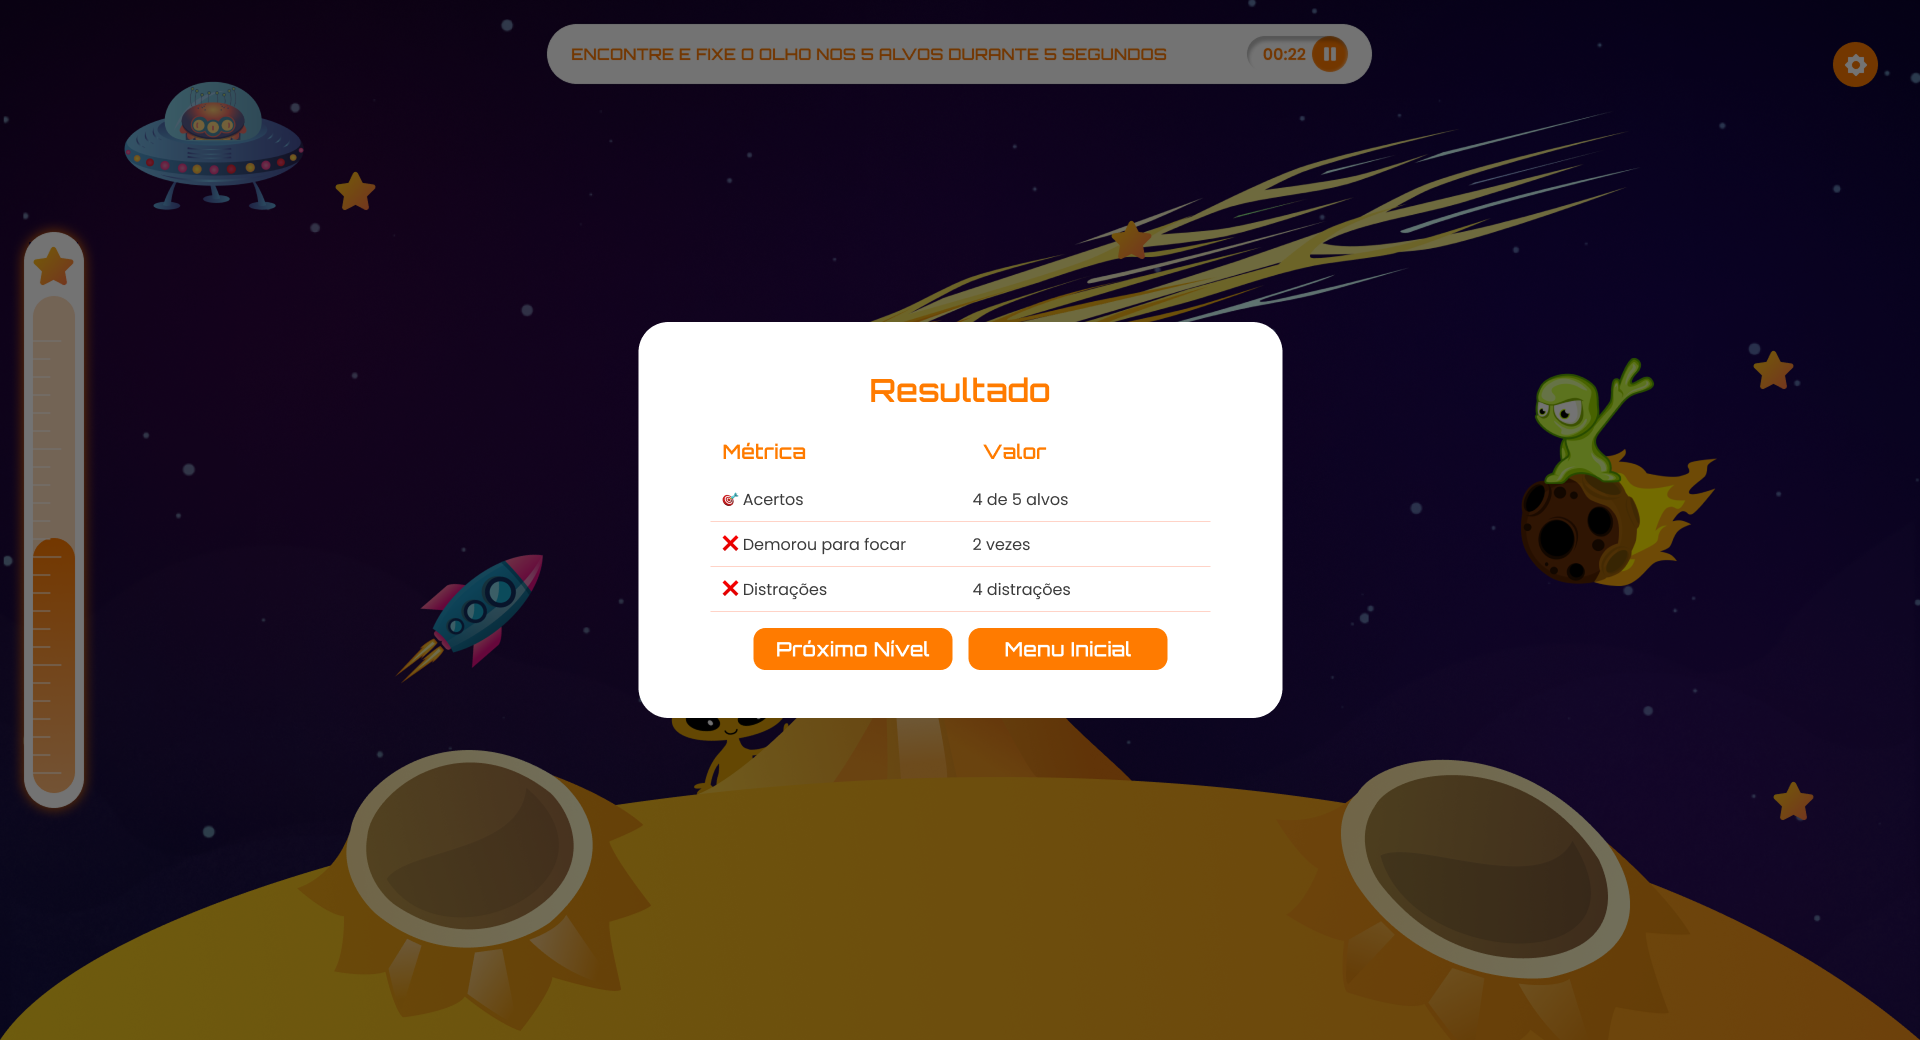
\includegraphics[width=\textwidth]{fim-primeira-fase.png}%
    \SourceOrNote{Autoria Própria (2025)}
\end{figure}

\begin{figure}[H]
    \centering
    \caption{Segunda fase}%
    \label{fig:segunda-fase}
    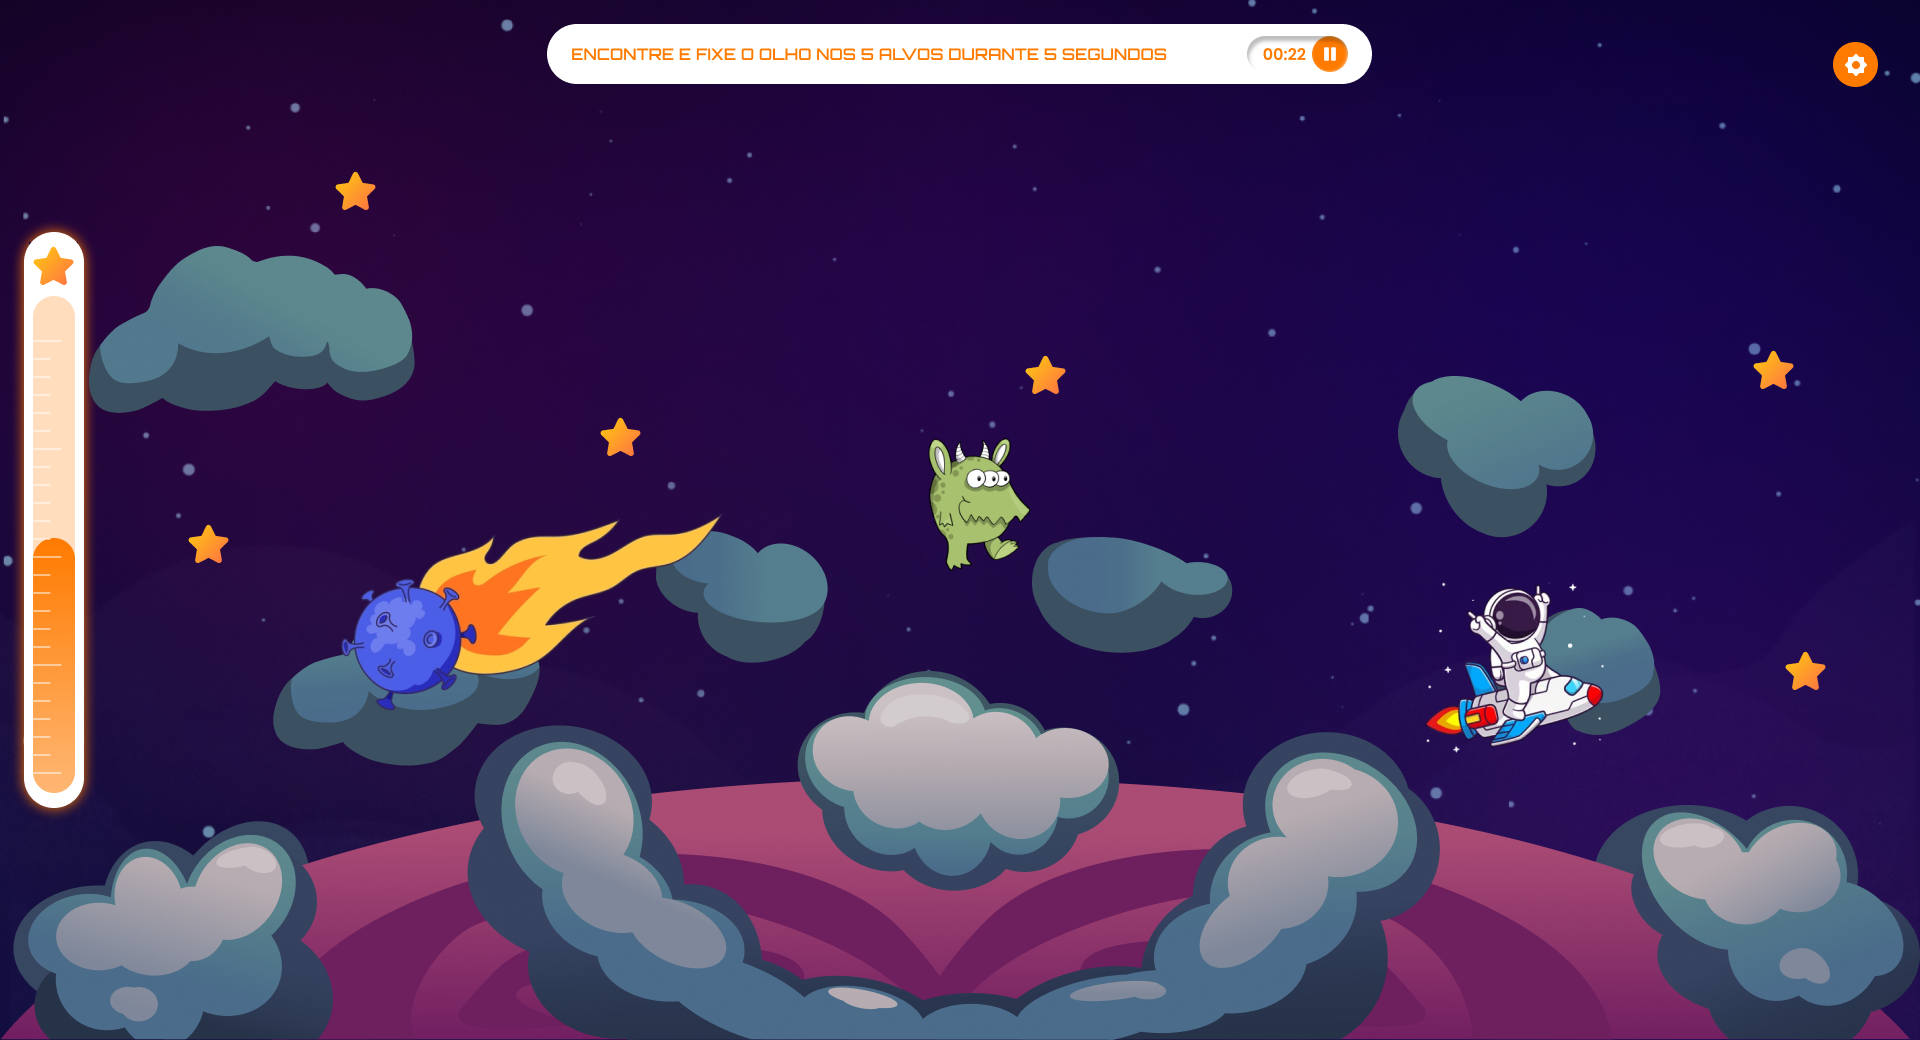
\includegraphics[width=\textwidth]{segunda-fase.png}%
    \SourceOrNote{Autoria Própria (2025)}
\end{figure}

Na segunda fase, o participante deve manter o foco em cinco estrelas estáticas, que brilham alternadamente (estímulo primário). Simultaneamente, três planetas em movimento transitam pela tela, atuando como distratores (estímulos secundários) cuja presença não é mencionada nas instruções. Essa abordagem foi escolhida por recomendação profissional. A fase 2 é composta por duas rodadas iguais de 15 segundos cada, nas quais apenas os planetas exibidos são alterados. Ao término de cada rodada, o participante é submetido a um teste de reconhecimento: sete opções de planetas são apresentadas, sendo que apenas três transitaram na tela. O participante deve indicar, por meio de botões IoT, quais planetas foram reconhecidos durante o trânsito. O reconhecimento correto de planetas efetivamente exibidos é contabilizado como acerto, enquanto a seleção de planetas não exibidos configura erro. Dessa forma, ao final da fase, são exibidas a quantidade de acertos, os planetas vistos e os planetas ignorados. O objetivo é avaliar a capacidade da criança de reconhecer os estímulos não citados nas instruções. A percepção dos planetas é tratada como um dado positivo para a inferência do pré-diagnóstico, pois contribui para a classificação do desempenho atencional da criança em relação aos resultados esperados. Por sua vez, a ausência de reconhecimento desses estímulos é considerada um dado complementar que também compõe a análise final, porém, negativamente. A trilha sonora, mais intensa e acelerada nesta fase, eleva a carga cognitiva e permite observar o impacto de múltiplos estímulos simultâneos na manutenção da atenção.

Nesta fase, foram aplicados procedimentos de atenção sustentada, isto é, manter o foco em um estímulo por um período prolongado. De acordo com a orientação profissional coletada na pesquisa qualitativa, o participante é instruído a concentrar-se nos alvos da tarefa e, ao final da fase, responde a uma pergunta adicional sobre a percepção dos planetas, apresentados como distrações. Além disso, a técnica proposta por // TODO: COLOCAR REF, na qual os participantes observam um fluxo contínuo de estímulos e respondem apenas a um sinal-chave, foi adaptada para investigar a percepção incidental de distrações sem alterar a ênfase principal na atenção sustentada.

No início da fase 2, uma conexão via WebSocket é aberta entre o cliente e o servidor. O servidor reconhece o cliente conectado, que apresenta estrelas piscando alternadamente enquanto planetas se movem pela tela. Ao final de cada rodada, o cliente envia ao servidor o comando de aguardo da resposta do usuário através do endpoint $\texttt{/aguardando\_iot}$. O servidor, então, transmite a mensagem ao IoT e solicita que acenda um LED, indicando que o participante pode responder. O IoT acende o LED e faz a leitura dos botões pressionados pelo evento $\texttt{button pressed}$. A cada clique no botão correspondente ao planeta, o IoT utiliza a função do servidor que envia ao cliente o planeta clicado e se ele está correto ou não. Se o planeta estiver correto, ele é iluminado com a cor verde; caso contrário, é iluminado com a cor vermelha. O participante pode apertar três botões por rodada. Ao finalizar ambas as rodadas, o servidor envia ao cliente a quantidade de acertos, planetas vistos e planetas ignorados através de $\texttt{/fase\_atual\_finalizada}$.

\begin{figure}[H]
    \centering
    \caption{Pergunta da segunda fase}%
    \label{fig:perguntas-segunda-fase}
    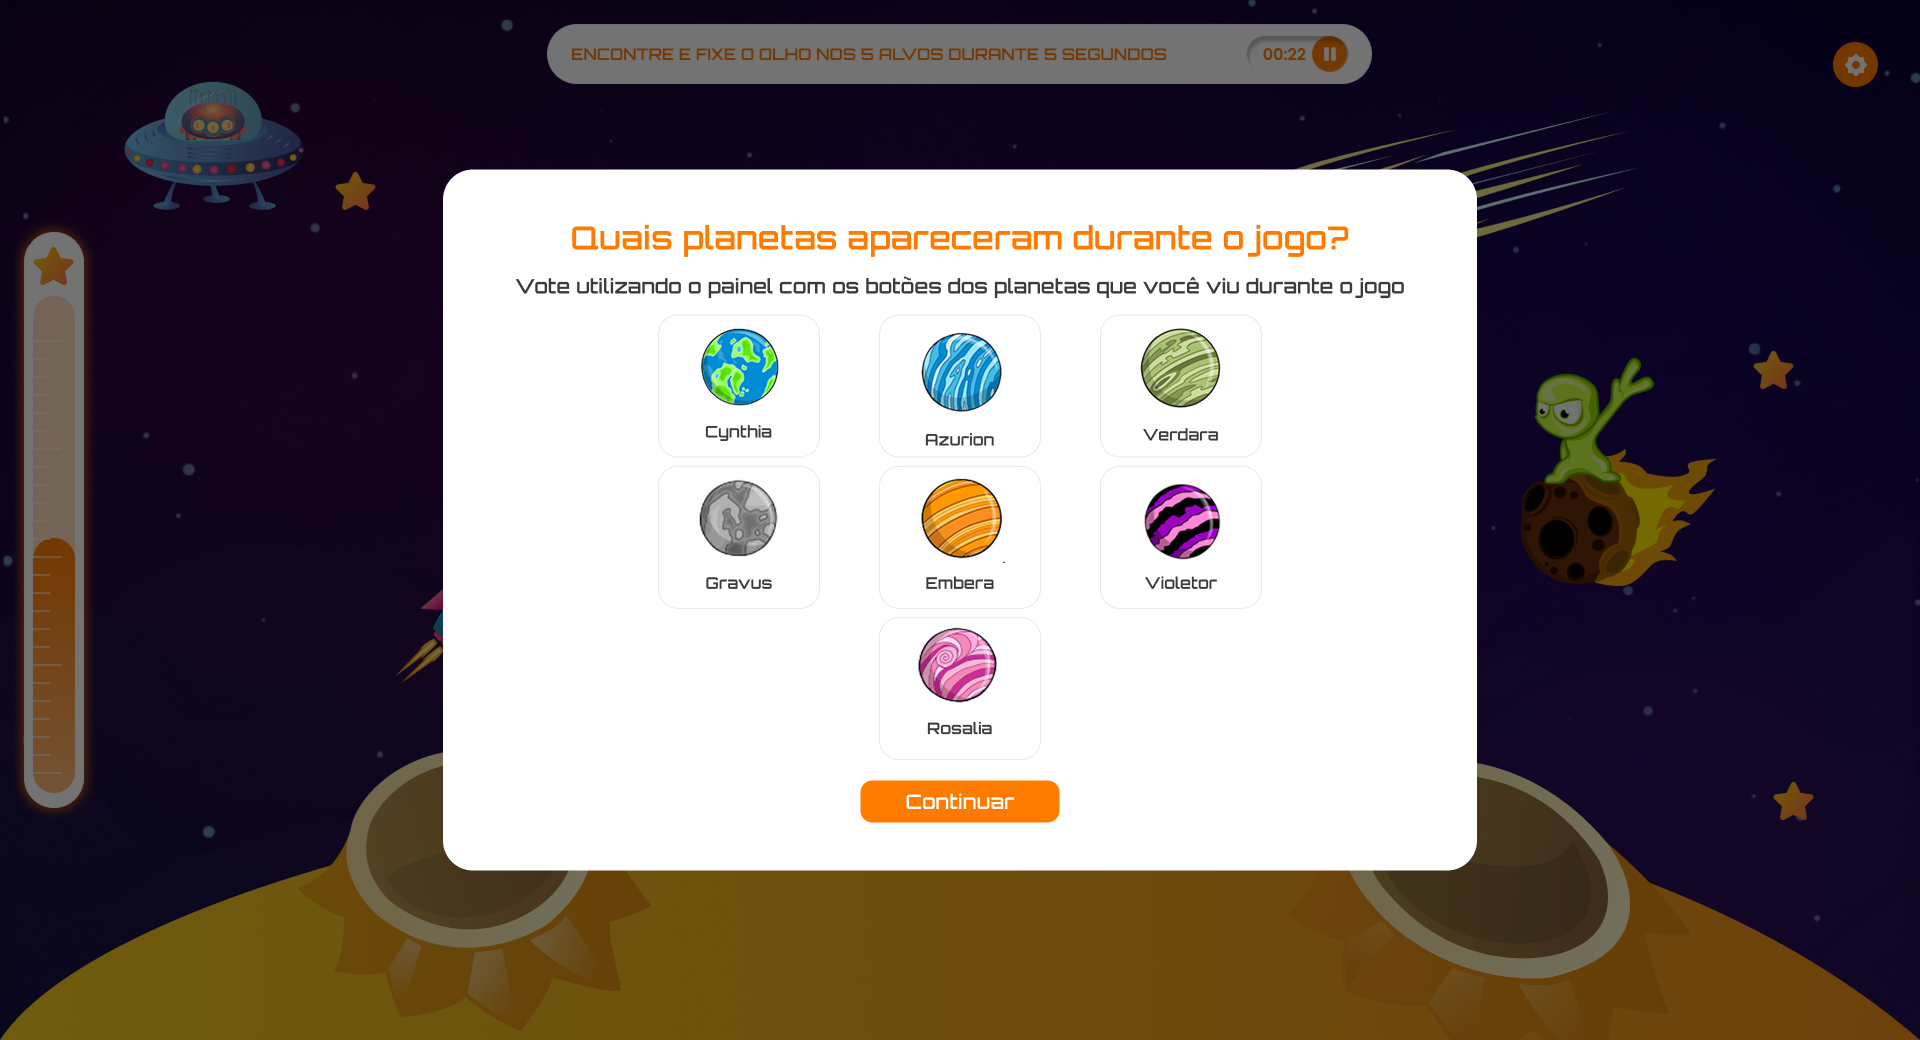
\includegraphics[width=\textwidth]{perguntas-segunda-fase.png}%
    \SourceOrNote{Autoria Própria (2025)}
\end{figure}

\begin{figure}[H]
    \centering
    \caption{Resultado da segunda fase}%
    \label{fig:fim-segunda-fase}
    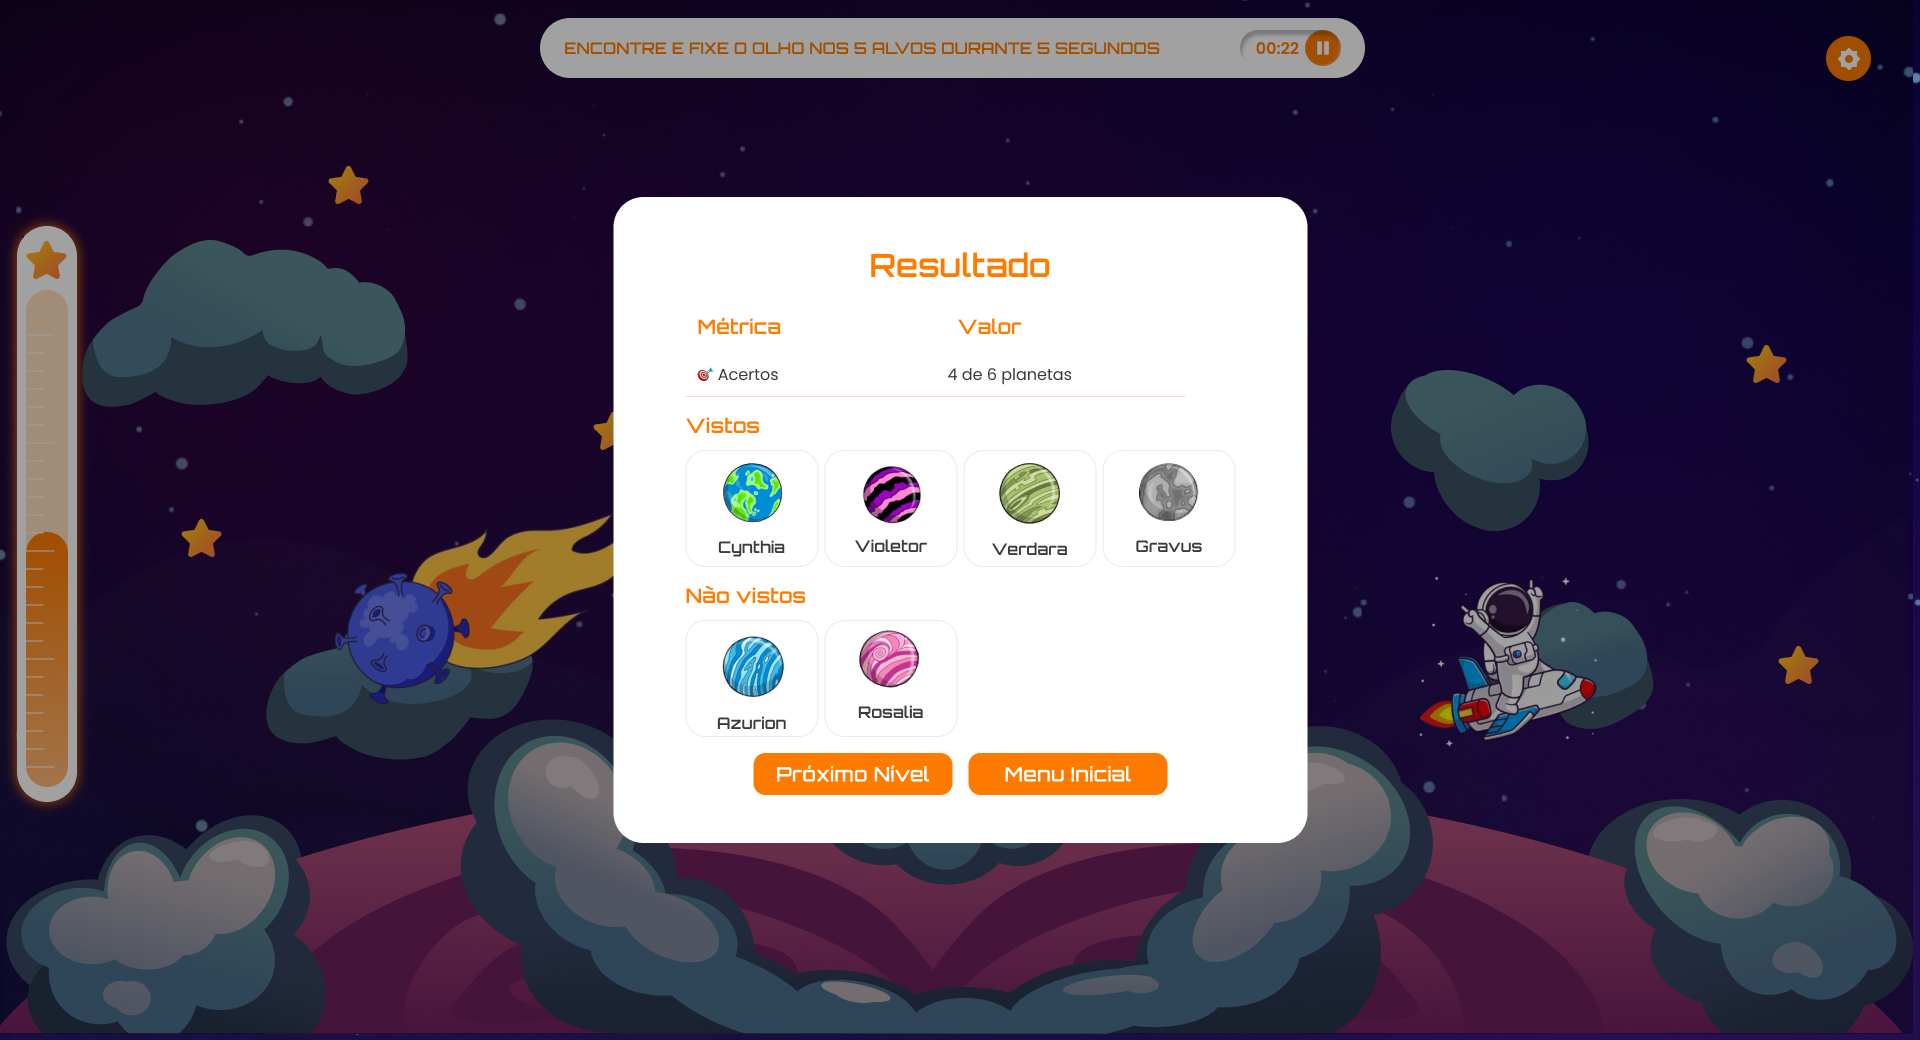
\includegraphics[width=\textwidth]{fim-segunda-fase.png}%
    \SourceOrNote{Autoria Própria (2025)}
\end{figure}

Para a construção do dispositivo de controle da IoT, foram empregados os seguintes componentes eletrônicos: uma placa de desenvolvimento Arduino, sete botões do tipo \textit{push-button}, sete resistores de 10 k$\Omega$, uma protoboard e cabos de conexão. Os botões foram conectados às portas digitais do Arduino, configuradas como entradas com resistores pull-down para garantir leituras estáveis. Dessa forma, ao término de cada rodada da segunda fase do jogo, o participante registra os planetas que conseguiu observar, pressionando o botão correspondente a ele. O Arduino atua como uma interface de comunicação de hardware, detectando o pressionamento físico dos botões IoT. Por meio da comunicação serial, o microcontrolador transmite o evento acionado ao sistema. O servidor é responsável por receber e interpretar este sinal do botão selecionado e, na sequência, acionar a função que contabiliza os acertos e os erros de inibição do participante para a fase.
// TODO: colocar foto do arduino 

Em futuras iterações do projeto, planeja-se o aperfeiçoamento estético e ergonômico do controle, por meio da substituição dos botões convencionais por peças personalizadas, modeladas em software CAD e fabricadas via impressão 3D, com design mais atrativo e ergonômico para crianças. Além disso, planeja-se construir uma case para o controle utilizando filamentos de garrafa PET, visando a sustentabilidade ambiental do projeto.
// TODO: colocar foto do arduino 3D

\begin{figure}[H]
    \centering
    \caption{Terceira fase}%
    \label{fig:terceira-fase}
    
\includegraphics[width=\textwidth]{terceira-fase.png}%
    \SourceOrNote{Autoria Própria (2025)}
\end{figure}

Na terceira fase, a demanda cognitiva é intensificada pela necessidade de alternância rápida do foco visual entre diferentes regiões da tela, caracterizadas por menor previsibilidade espacial. Nessa etapa, uma estrela surge de forma estática, exigindo resposta ocular imediata do participante. Simultaneamente, um segundo estímulo estático é apresentado (radar de uma aeronave), alternando entre os estados ligado e desligado em intervalos regulares. Quando esse estímulo é ativado (ascende), o participante deve manter o olhar fixo sobre ele até que se apague, o que permite avaliar a atenção dividida e o controle do direcionamento ocular. Além disso, aplicou-se a técnica // TODO: COLOCAR REF, onde os participantes observam um fluxo contínuo de estímulos e respondem apenas a um sinal-chave (estrela ou radar acesos), sendo que a resposta deve ser direcionada ao alvo previsto. A duração desta fase é de 30 segundos. A trilha sonora atinge seu nível máximo de intensidade e agitação, contribuindo para aumentar a complexidade da tarefa. O desempenho do participante nesta fase é utilizado como indicador da agilidade atencional e da capacidade de redirecionamento e manutenção do foco visual diante de estímulos dinâmicos. Ao fim da terceira fase, métricas como número de acertos (fixação por 5 segundos), número de erros de omissão (demora de 10 segundos ou mais para iniciar a fixação) e erros de comissão (início da fixação antes de 10 segundos, sem manutenção do foco por 5 segundos) são calculados e apresentados ao participante, conforme ilustrado na Figura \ref{fig:fim-terceira-fase}.

\begin{figure}[H]
    \centering
    \caption{Resultado da terceira fase}%
    \label{fig:fim-terceira-fase}
    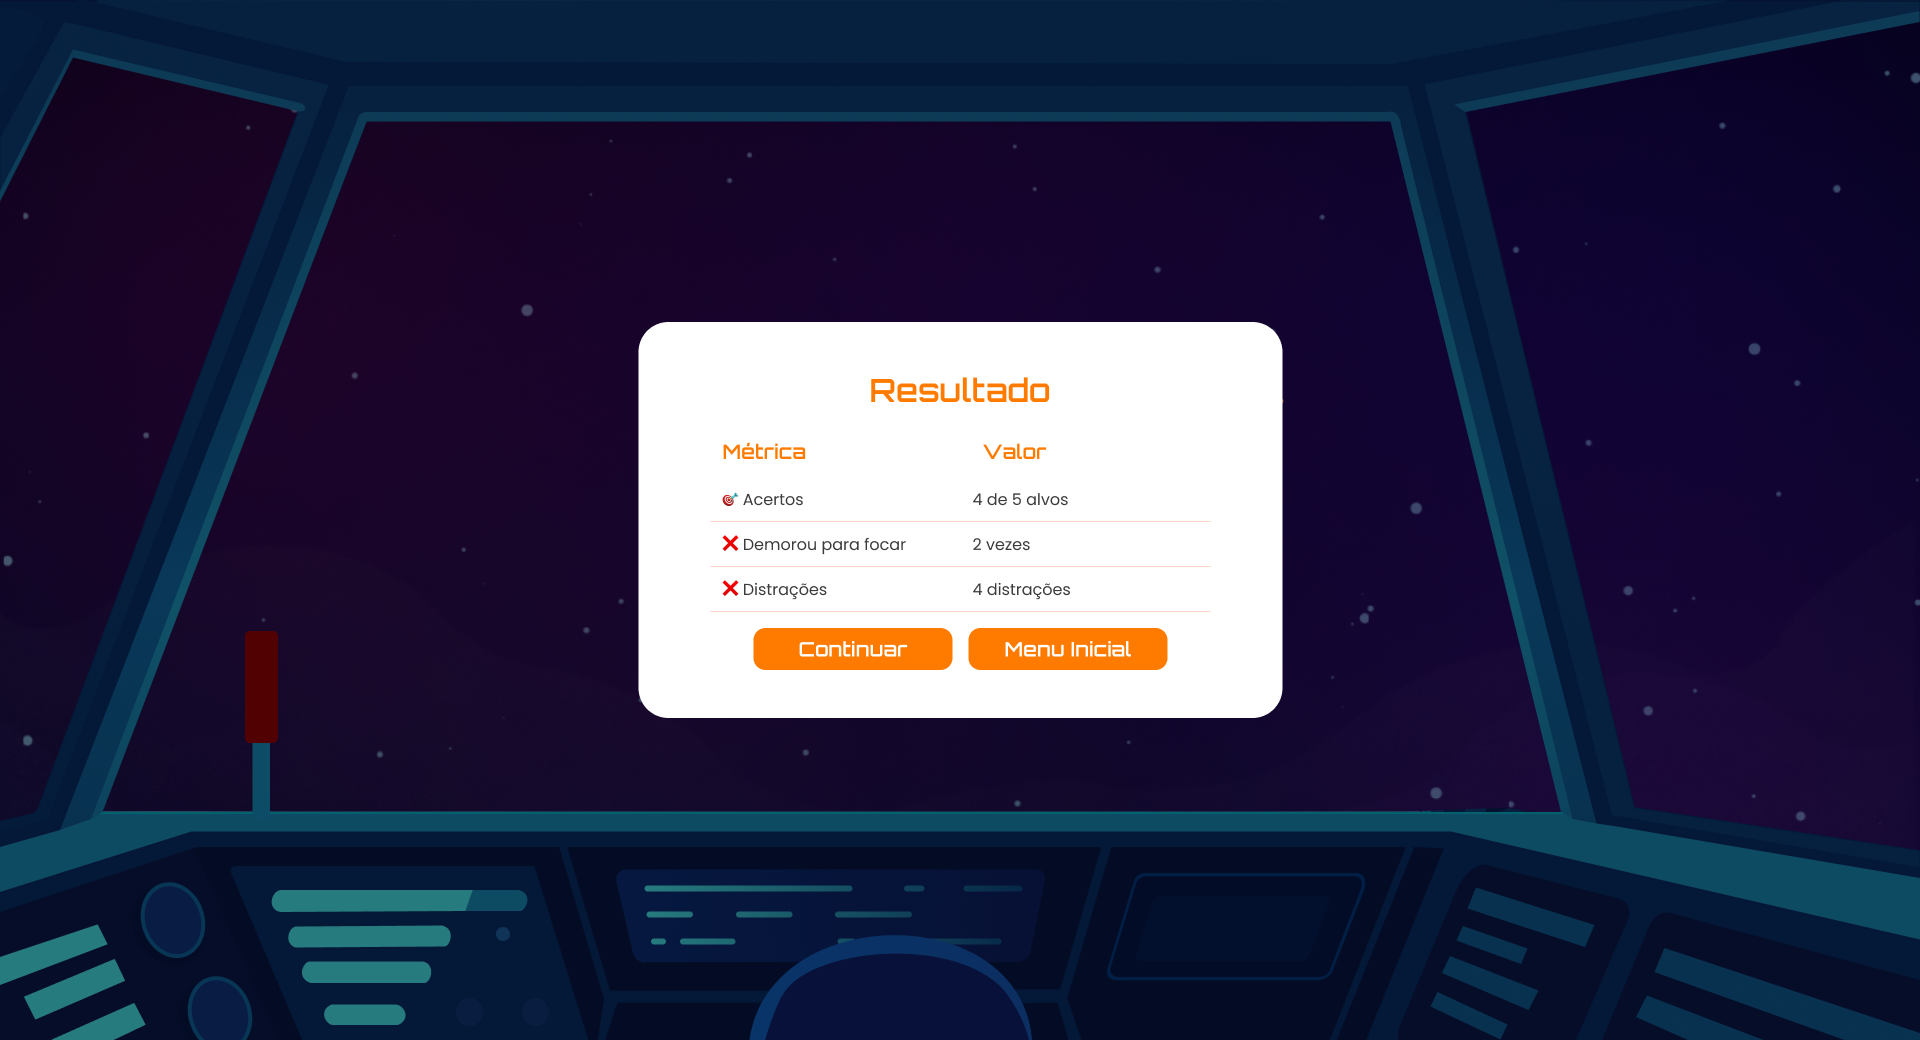
\includegraphics[width=\textwidth]{fim-terceira-fase.png}%
    \SourceOrNote{Autoria Própria (2025)}
\end{figure}

// TODO: ADD EXPLICAÇÃO DO CÓDIGO DA TERCEIRA FASE

Ao término das três fases, o sistema irá gerar um pré-diagnóstico com base nas métricas TDC. Para isso, serão utilizados os registros de desempenho e os dados mais recentes de rastreamento ocular obtidos durante as fases, sendo eles: acertos, erros de omissão, erros de comissão, tempo de resposta e desvio padrão. Este pré-diagnóstico será elaborado por um módulo de IA, que interpreta as métricas e o desempenho do participante. O feedback resultante é apresentado em duas formas: (1) uma mensagem textual interpretativa, como: “Sua atenção está conforme o esperado”, “Sua atenção está acima do esperado” ou “Sua atenção está abaixo do esperado”, de acordo com o desempenho observado; e (2) a exibição de uma porcentagem que representa a precisão do olhar capturada pelo sistema de rastreamento ocular, conforme ilustrado na Figura \ref{fig:fim-geral}.

\begin{figure}[H]
    \centering
    \caption{Pré-diagnóstico}%
    \label{fig:fim-geral}
    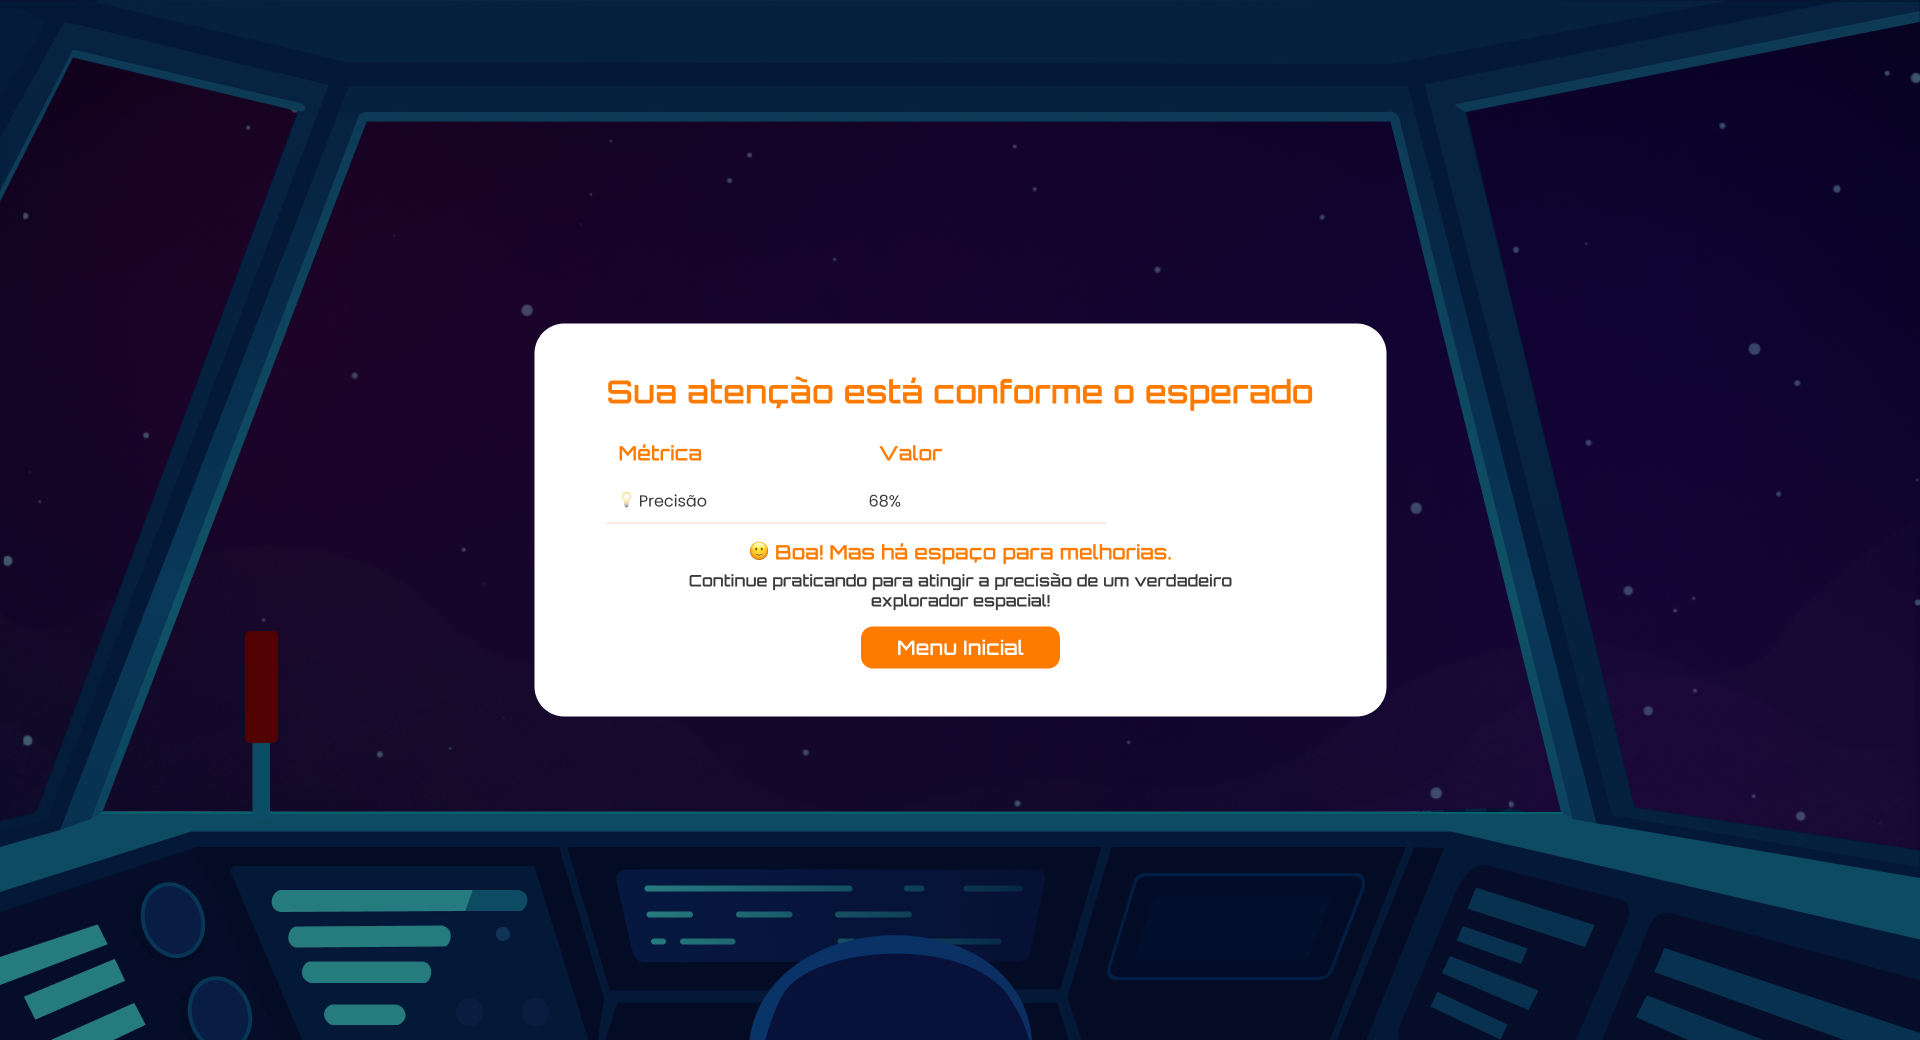
\includegraphics[width=\textwidth]{fim-geral.png}%
    \SourceOrNote{Autoria Própria (2025)}
\end{figure}

Considerando a análise realizada pelo profissional e os resultados a serem apresentados aos pais ou responsáveis, o pré-diagnóstico é disponibilizado em relatório com linguagem clara, acessível e visualmente intuitiva. A mensagem interpretativa é redigida sem termos técnicos, de modo a oferecer uma avaliação direta do desempenho da criança em relação aos padrões esperados. A Figura \ref{fig:relatorio} exemplifica o layout e o conteúdo do relatório gerado pelo sistema, que visa facilitar a compreensão dos resultados e orientar as decisões futuras.

\begin{figure}[H]
    \centering
    \caption{Relatório de Pré-diagnóstico}%
    \label{fig:relatorio}%
    
\includegraphics[width=\textwidth]{relatorio.png}%
    \SourceOrNote{Autoria Própria (2026)}
\end{figure}

A plataforma foi desenvolvida com tecnologias web, possibilitando acesso remoto e execução direta em \textit{browsers}, preferencialmente com a webcam Logitech Brio Cam HS, por apresentar melhor qualidade na captura do olhar. Optou-se pela plataforma web considerando-se múltiplos fatores: a estabilidade do equipamento durante a calibração e execução das fases do jogo; o contexto de uso destinado a crianças, para o qual um dispositivo móvel poderia resultar em desatenção ou menor comprometimento, ao ser confundido com uma atividade comum de entretenimento; a temática espacial com abundância de elementos visuais, que exigiria redução dimensional em telas móveis, prejudicando a disposição adequada dos elementos; e, finalmente, o contexto de aplicação por profissionais em ambientes de escritório, onde notebooks são mais disponíveis. O teste é executado em ambiente silencioso, sob supervisão de profissional responsável pela preparação do ambiente, criação do perfil da criança e orientação do procedimento, conforme as instruções disponibilizadas pela plataforma. 

No projeto atual, a IA será utilizada para análisar os dados coletados durante o jogo, referentes aos erros e acertos, com uma base de dados previamente formada por indivíduos diagnosticados com TDA e por outros sem o transtorno. Entretanto, nesta fase inicial de desenvolvimento, é necessário testar a viabilidade do sistema. Inicialmente, dez crianças com TDA serão convidadas a participar do experimento, com o objetivo de coletar dados iniciais que servirão como base para o treinamento supervisionado do modelo de IA. Em seguida, três crianças com TDA e três sem o transtorno (diferentes das 10 iniciais, ou seja, ainda não analisadas) 
serão convidadas para uma nova etapa experimental, destinada a validar a eficácia do sistema na identificação de indícios de desatenção. O objetivo é garantir que a acurácia do sistema seja satisfatória antes de ampliar a base de dados e aperfeiçoar o modelo. Após a conclusão da fase de validação, o sistema estará apto a ser utilizado por um público mais amplo, contribuindo para a identificação precoce do TDA em crianças e reforçando seu potencial como ferramenta de apoio ao diagnóstico. 

No que se refere à retroalimentação da IA, o sistema irá conter um modo de treinamento, que pode ser ativado ou desativado exclusivamente pelo administrador. A mecânica dessa funcionalidade é empregada sempre que houver necessidade de alimentar a base de dados com novos registros. Essa etapa só pode ser executada na presença de ao menos um administrador, a fim de garantir a integridade e a qualidade dos dados inseridos. Caso contrário, a criança participa normalmente do jogo apenas para avaliar seu nível de atenção. Quando o modo de treinamento está habilitado, o sistema armazena as métricas TDC coletadas durante as partidas em uma base de dados, permitindo que o módulo de treinamento da IA realize a análise comparativa entre os dados do indivíduo e a base existente. Esse processo tem como objetivo retroalimentar o modelo e aperfeiçoar continuamente o desempenho da IA. 

% Resultados e Discussões
\section{Resultados e Discussões}

\lipsum[12-13] Os resultados obtidos demonstram a eficácia da metodologia proposta. A Tabela \ref{tab:resultados} apresenta uma comparação quantitativa entre diferentes abordagens.

\begin{table}[H]
\centering
\caption{Comparação de desempenho entre diferentes métodos}
\label{tab:resultados}
\begin{tabular}{@{}lccc@{}}
\toprule
\textbf{Método} & \textbf{RMSE} & \textbf{Tempo (s)} & \textbf{Precisão (\%)} \\ \midrule
Método Proposto & 0.0023 & 15.2 & 98.5 \\
Euler Clássico & 0.0145 & 8.7 & 92.3 \\
Runge-Kutta 4ª ordem & 0.0038 & 21.5 & 97.1 \\
Método Adaptativo & 0.0031 & 18.9 & 97.8 \\ \bottomrule
\end{tabular}
\end{table}

\subsection{Análise Quantitativa}

\lipsum[14] Os dados quantitativos revelam que o método proposto apresenta melhor desempenho em termos de precisão. A relação entre os parâmetros pode ser expressa por:

\begin{equation}
\eta = \frac{P_{out}}{P_{in}} \times 100\% = \frac{V_{out} \cdot I_{out}}{V_{in} \cdot I_{in}} \times 100\%
\label{eq:efficiency}
\end{equation}

onde $\eta$ representa a eficiência do sistema, $P_{out}$ é a potência de saída e $P_{in}$ é a potência de entrada.

\subsection{Análise Qualitativa}

\lipsum[15] Do ponto de vista qualitativo, observou-se que o comportamento do sistema é fortemente influenciado pelas condições iniciais e pelos parâmetros de controle. A matriz de transformação pode ser representada como:

\begin{equation}
\mathbf{A} = \begin{bmatrix}
a_{11} & a_{12} & a_{13} \\
a_{21} & a_{22} & a_{23} \\
a_{31} & a_{32} & a_{33}
\end{bmatrix}
\label{eq:matrix}
\end{equation}

\subsection{Discussão}

\lipsum[16-17] A análise dos resultados indica que a abordagem proposta oferece vantagens significativas em relação aos métodos tradicionais. Lorem ipsum dolor sit amet, consectetur adipiscing elit. Nullam in dui mauris. Vivamus hendrerit arcu sed erat molestie vehicula.

Proin adipiscing porta tellus, ut feugiat nibh adipiscing sit amet. In eu justo a felis faucibus ornare vel id metus. Vestibulum ante ipsum primis in faucibus orci luctus et ultrices posuere cubilia curae.

% Conclusão
\section{Conclusão}

Este trabalho teve como foco o desenvolvimento de uma solução tecnológica como auxílio ao pré-diagnóstico de indícios de TDA em crianças entre 10 e 12 anos, por meio da integração entre rastreamento ocular, métricas do Teste de Desempenho Contínuo, \textit{IoT} e IA.

Os resultados obtidos demonstram que a solução funciona na etapa atual do projeto. O jogo foi implementado, integrado aos módulos de coleta de dados oculares em tempo real e capaz de gerar retorno inicial sobre o desempenho atencional dos participantes a partir do processamento automático dos dados. 

No módulo de rastreamento ocular, observou-se precisão satisfatória para a fase atual, confirmando a viabilidade técnica da abordagem. Em relação às métricas TDC, a aplicação foi adequada durante os testes realizados. Por fim, no componente de \textit{IoT}, o funcionamento foi adequado e promissor durante os testes. Entretanto, permanecem pontos de melhoria já identificados: aumento da robustez e da estabilidade da predição ocular em diferentes condições de uso, por meio de estudos de bibliotecas e técnicas de \textit{eye tracking}; aperfeiçoamento ergonômico do \textit{case} físico do dispositivo; e implementação do módulo de IA, cuja consolidação depende da confiabilidade dos dados de rastreamento ocular de entrada.

Como continuidade do estudo, devem ser realizados testes em ambiente controlado com profissionais da saúde e crianças da faixa etária-alvo, além da validação progressiva dos modelos de IA para identificação de padrões e emissão de relatórios detalhados. Conclui-se, portanto, que a proposta desenvolvida apresenta aplicabilidade prática e potencial de contribuição para auxiliar na identificação de indícios de TDA, ao mesmo tempo em que requer aprimoramentos incrementais para atingir maior maturidade técnica e operacional.

% Agradecimentos
\section*{Agradecimentos}

Os autores agradecem à Faculdade de Tecnologia do Estado de São Paulo (FATEC) e ao Centro Paula Souza (CPS) pelo apoio institucional. 
% Este trabalho foi parcialmente financiado pela FAPESP (proc. 2024/12345-6) e CNPq (proc. 301234/2024-0).

% Referências
\bibliographystyle{IEEEtran}
\bibliography{referencias}

\end{document}
